\documentclass[a4paper]{article}

\title{PH2255 Course:\\
Quantum Harmonic Oscillators}
\author{Thomas Bass}
\date{27 March 2021}

% LaTeX preambule: loading relevant packages, configuring Python listings
\usepackage{graphicx}
\usepackage{amsmath}
\usepackage{color}
\usepackage{listings}
\usepackage{hyperref}
\usepackage{bm}
\usepackage{physics}
\usepackage{subcaption}
\usepackage[a4paper, total={6in, 8in}]{geometry}




\definecolor{dkgreen}{rgb}{0,0.6,0}
\definecolor{gray}{rgb}{0.5,0.5,0.5}
\definecolor{mauve}{rgb}{0.58,0,0.82}

% Settings for colour-coding and formatting Python code:
\lstset{
  language=Python,                % the language of the code
  basicstyle=\footnotesize,           % the size of the fonts that are used for the code
  numbers=left,                   % where to put the line-numbers
  numberstyle=\tiny\color{gray},  % the style that is used for the line-numbers
  stepnumber=5,                   % the step between two line-numbers. If it's 1, each line
                                  % will be numbered
  numbersep=5pt,                  % how far the line-numbers are from the code
  backgroundcolor=\color{white},      % choose the background color. You must add \usepackage{color}
  showspaces=false,               % show spaces adding particular underscores
  showstringspaces=false,         % underline spaces within strings
  showtabs=false,                 % show tabs within strings adding particular underscores
  frame=single,                   % adds a frame around the code
  rulecolor=\color{black},        % if not set, the frame-color may be changed on line-breaks within not-black text (e.g. commens (green here))
  tabsize=2,                      % sets default tabsize to 2 spaces
  captionpos=b,                   % sets the caption-position to bottom
  breaklines=true,                % sets automatic line breaking
  breakatwhitespace=false,        % sets if automatic breaks should only happen at whitespace
  title=\lstname,                   % show the filename of files included with \lstinputlisting;
                                  % also try caption instead of title
  keywordstyle=\color{blue},          % keyword style
  commentstyle=\color{dkgreen},       % comment style
  stringstyle=\color{mauve},         % string literal style
  escapeinside={\%*}{*)},            % if you want to add LaTeX within your code
  morekeywords={*,...}               % if you want to add more keywords to the set
}

\begin{document}
\maketitle

\begin{abstract}
%%%%%%
TODO
%%%%%%
\end{abstract}

\section{Hooke's Law and the Quantum Harmonic Oscillator}
To begin an analysis of quantum harmonic oscillators (QHO), we begin with Hooke's law. While this law is in the classical regime, later it can be proved\footnote{In Section \ref{section:bohr}} that we can apply the same potentials described by Hooke's spring model to the forces experienced by an atom in equilibrium. By differentiating Hooke's law we can obtain the work done by displacing the mass:
\begin{equation} \label{eq:hooke}
W.D.=V(x)=\frac12kx^2=\frac12m\omega^2x^2
\end{equation}
Then, by substituting this potential into the 1D Schr\"odinger Equation, we obtain the equation for our QHO:
\begin{equation} \label{eq:tise}
\frac{-\hbar^2}{2m}\nabla^2\psi(x) + \frac12m\omega^2_cx^2\psi(x)=E\psi(x)
\end{equation}
We then substitute the displacement $x$ and energy $E$ for dimensionless variables, using the reduced Planck constant:
\begin{equation} \label{eq:xsub}
y=\frac xa=\sqrt{\frac{m\omega_c}\hbar}\cdot x
\end{equation}
\begin{equation} \label{eq:Esub}
\varepsilon=\frac E{\hbar\omega_c/2}
\end{equation}
By substituting Equations \ref{eq:xsub} and \ref{eq:Esub} into Equation \ref{eq:tise}, we obtain a homogeneous equation, for which we can solve
\begin{equation} \label{eq:tise_hom}
\nabla^2\psi(y)+(\varepsilon-y^2)\psi(y)=0
\end{equation} 
\newpage
\section{Hermite Polynomials}
To solve the differential equation \ref{eq:tise_hom}, we use a trial solution  $\psi_n(y)=H_n(y)\cdot\exp(-y^2/2)$, where $H_n$ is a function to be determined. From a brief analysis, we can see that the exponential term will survive differentiation, and that it will cancel out with the negative $y^2$ term. By  taking the second derivative, we obtain:
\begin{equation}
\psi''(y)=[H''-2yH'+H(y^2-1)]\cdot e^{-y^2/2}
\end{equation}
We substitute this into Equation \ref{eq:tise_hom}, and obtain:
\begin{equation}
\psi''(y)+(\varepsilon-y^2)\psi(y)=[H''-2yH'+(\varepsilon-1)H]\cdot e^{-y^2/2}=0
\end{equation}
As the exponential term is always great than zero, we must solve the square-bracketed terms for zero. These are the Hermite polynomials\footnote{Discussed in detail in \cite[\S1T1 $\sim$ p.57 ]{RefWorks:doc:606076f48f081b19e4859e9a}}, and are defined by:
\begin{equation}
H(y)=\sum^\infty_{p=0}a_py^p=a_0+a_1y+a_2y^2+...
\end{equation}
As these polynomials are now in a computable form, we can rewrite our general solution, converting back to the variable $x$:
\begin{equation}
\psi(x)=\frac{H_n(x/a)}{\sqrt{2^nn!\sqrt{\pi a^2}}}e^{-\frac{x^2}{2a^2}}
\end{equation}
This then provides us with a general solution to our QHO, which we can easily compute using Python.

\section{Ground State Analysis}
In the ground state, $\psi_0(x)$, we expect to see the normal probability distribution for our wave function. The $0^\text{th}$ order Hermite polynomial is given as $H_0(y)=1$, which provides us with a simple wave function:
\begin{equation}
\psi_0(x)=\frac1{(\pi a^2)^{1/4}}e^{-x^2/2a^2}
\end{equation}
For the probability density of the ground state, we take the absolute square of the wave function $p_0(x)=|\psi_0(x)|^2$. By plotting these in Python, we can see that this result follows the expected normal distribution.
\begin{figure}[h!]
\centerline{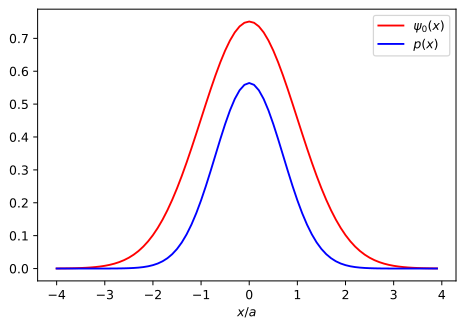
\includegraphics[scale=0.7]{ground_state.png}}
\caption{Graph showing the energy of the ground state wave function, and its probability density.}
\label{fig:ground_state}
\end{figure}
From these graphs, we can see that the ground state wave function $\psi_0(x)$ is an even function.

\subsection{Orthogonality}
To apply the position and momentum operators to the wave function, we must first verify that it is normalised and orthogonal. To verify orthogonality of normalised eigenfunctions, we use the inner product, as defined in \cite[\S3.1.2$\sim$p.25]{RefWorks:doc:60607bf68f08266f5a4c455d}:
\begin{equation}
\bra{\psi_m} \ket{\psi_n} =\int^\infty_{-\infty}\psi^*_n(x)\psi_m(x)dx = \delta_{mn}
\end{equation}
Where $\delta_{ij}$ is the Kronecker delta function:
\begin{equation}
{\displaystyle \delta _{ij}={\begin{cases}0&{\text{if }}i\neq j,\\1&{\text{if }}i=j.\end{cases}}}
\end{equation}
To verify this, we use the \lstinline$integrate.quad$ method provided by Python's SciPy library. By constructing a function \lstinline$psi(x, n)$ in python, analogous to $\psi_n(x)$, we can calculate the inner product as the integral:
\begin{equation}
\bra{\psi_0} \ket{\psi_n}=\int^\infty_{-\infty}\psi_0^*(x)\psi_n(x)dx
\end{equation}
For $\psi_n(x)$ wave functions of $n=1, 3, 4, 7$.
\begin{lstlisting}
for i in [1, 3, 4, 7]:
    inner_product = integrate.quad(np.vectorize(lambda x: psi(x, 0)*psi(x, i)), -float("inf"), float("inf"))[0]
\end{lstlisting} As the wave functions are not complex, we use $\psi^*=\psi$. This numerical integration method verifies the orthogonality of the ground state wave function. The result for $\bra{\psi_m} \ket{\psi_4}$ is calculated as \lstinline$-6.106226635438361e-16$, but this is disregarded as a floating-point inaccuracy, as all other values of $n$ return precisely zero.

\subsection{Position operator} \label{section:position}
To calculate the uncertainty of position for the wave function, we employ the position operator $\hat x=x$ to calculate the expectation value of the position observable. 
\begin{equation}
\expval x=\mel{\psi_0}{\hat x}{\psi_0}=\int^\infty_{-\infty}\psi_0^*(x)\ x\ \psi_0(x)dx
\end{equation}
We once again use the \lstinline$integrate.quad$ method in Python:
\begin{lstlisting}
expectation_x = integrate.quad(np.vectorize(lambda x: psi(x, 0)*x*psi(x, 0)), -float("inf"), float("inf"))[0]
\end{lstlisting} This returns the value $\mel{\psi_0}{\hat x}{\psi_0}=0$, as we expected to obtain from the even parity of the probability density $|\psi_0(x)|^*$.
To find the position-squared expectation value, $\expval{x^2}$, we use a similar code snippet, replacing \lstinline$x$ with \lstinline$x**2$, from which we obtain the value \lstinline$0.5000000000000012$. Again, we round this to 0.5 to account for floating point inaccuracy . By varying our value of $a$, we obtain the following values for $\expval{x^2}$.
\begin{table}[h!]
\centering
\begin{tabular}{cc}
a & $\expval x^2$ \\ \hline
1 & 0.5000000000000012  \\
2 & 0.25000000000000056 \\
3 & 0.16666666666666707
\end{tabular}
\caption{\label{tab:expect}Values of $\expval x^2$ calculated using SciPy's numerical integration function.}
\end{table}

From these values, we can readily see that the expected value $\mel{\psi_0}{\hat x^2}{\psi_0} = a^2/2$ is obtained.

\subsection{Momentum Operator} \label{section:momentum}
To calculate the momentum uncertainties, we now employ the momentum operator $\hat p=-i\hbar\nabla$ to calculate the momentum expectation value $\expval p$.
\begin{equation}
\expval p=\mel{\psi_0}{\hat p}{\psi_0}=-i\hbar\int^\infty_{-\infty}\psi_0^*(x)\ \frac\partial{\partial x} \psi_0(x)dx
\end{equation}

To compute this derivative, we use another method provided by SciPy, \lstinline$misc.derivative$, assigning a temporary callable variable for $\psi_0(x)$. 
\begin{lstlisting}
def psi0(x): return psi(x, 0)

expectation_p = hbar*1j*integrate.quad(np.vectorize(lambda x : psi0(x) * derivative(psi0, x, dx=0.0001, n=1)), -float("inf"), float("inf"))[0]
\end{lstlisting} This gives us the expected result of $\mel{\psi_0}{\hat p}{\psi_0}=0$.
To find the momentum-squared expectation value $\expval{p^2}$, we modify the above code snippet to produce the second order derivative, using \lstinline$n=2$:
\begin{equation}
\expval {p^2}=\mel{\psi_0}{\hat p^2}{\psi_0}=-\hbar^2\int^\infty_{-\infty}\psi_0^*(x)\ \frac{\partial^2}{\partial x^2} \psi_0(x)dx
\end{equation}
\begin{lstlisting}
expectation_p_sq = -hbar**2*integrate.quad(np.vectorize(lambda x : psi0(x) * derivative(psi0, x, dx=0.0001, n=2)), -float("inf"), float("inf"))[0]
\end{lstlisting} From which we obtain a value of \lstinline$0.49999999789637256$, rounded to 0.5 for floating point accuracy. By once again varying our value of $a$, we can obtain a formula for $\expval{p^2}$ in terms of $a$ and $\hbar$.
\begin{table}[h!]
\centering
\begin{tabular}{cc}
a & $\expval x^2$ \\ \hline
1 & 0.49999999789637256  \\
2 & 0.10937499999999994 \\
3 & 0.03497942386831273
\end{tabular}
\caption{\label{tab:p_table}Values of $\expval p^2$ calculated using SciPy's numerical integration function.}
\end{table}

From Table \ref{tab:p_table}, we can show that $\mel{\psi_0}{\hat p^2}{\psi_0}$ matches the expected equation $\hbar^2/2a^2$.
\newpage
\subsection{Calculating Uncertainties}
Now that we have calculated the expectation values for position and momentum, , we can calculate the uncertainties $\Delta x$ and $\Delta p$ for position and momentum. Reference \cite[\S3.3$\sim$p.123]{RefWorks:doc:60607e6a8f08266f5a4c458e} provides us with an equation relating the expectation values of a system to the standard deviation of these observables:
\begin{equation}
\Delta A=\sqrt{\expval{(A-\expval A)^2}}
\end{equation}
With some simple commutator algebra, we arrive at the following equations describing the uncertanties for position and momentum:
\begin{equation}\label{eq:Dx}
(\Delta x)^2=\expval{x^2}-\expval x^2
\end{equation}
\begin{equation}\label{eq:Dp}
  (\Delta p)^2=\expval{p^2}-\expval p^2
\end{equation}
Therefore, by using the expectation values we calculated in Sections \ref{section:position} and \ref{section:momentum}, we can derive the uncertainties $\Delta x$ and $\Delta p$ for position and momentum:
\begin{equation}
\Delta x = \sqrt{\expval{x^2}-\expval x^2} = \sqrt{ \frac{a^2}2 -0^2}=\frac a{\sqrt 2}
\end{equation}
\begin{equation}
\Delta p = \sqrt{\expval{p^2}-\expval p^2} = \sqrt{ \frac{\hbar^2}{2a^2} -0^2}=\frac\hbar{\sqrt 2 a}
\end{equation}
From these, we can easily arrive at the expected expression for the Heisenburg Uncertainy Principle \cite[Eq.63$\sim$p.113]{RefWorks:doc:606076f48f081b19e4859e9a}:
\begin{equation} \label{eq:dxdp}
\Delta x\Delta p=\frac a{\sqrt2}\cdot\frac\hbar{\sqrt2a}=\frac\hbar2
\end{equation}

\section{n$>$0 Analysis}
\subsection{Position and Momentum Expectation Values, and Uncertainties}
To verify these results for wave functions $\psi_n(x)$ above the ground state, we modify the existing code and iterate over wave functions for $n=0, 1, ..., 10$\footnote{See Appendix \ref{sec:python}}. The results of these calculations are tabulated below. 
  \begin{table}[h!]
  \centering
  \begin{tabular}{cccc}
  n     & $\Delta x_n$       & $\Delta p_n$       & $\approx\Delta x_n\Delta p_n$ \\\hline
  0     & 0.7071067811865483 & 0.7071067796990583 & $1/2$ \\
  1     & 1.2247448713915887 & 1.2247448710189657 & $3/2$ \\
  2     & 1.5811388300841895 & 1.5811388282180328 & $5/2$ \\
  3     & 1.8708286933869707 & 1.8708286880893845 & $7/2$ \\
  4     & 2.1213203435596424 & 2.1213203376391427 & $9/2$ \\
  5     & 2.345207879911715  & 2.345207872688048  & $11/2$ \\
  6     & 2.5495097567963927 & 2.5495097437877368 & $13/2$ \\
  7     & 2.738612787525834  & 2.738612774744414  & $15/2$ \\
  8     & 2.915475947422669  & 2.915475933768039  & $17/2$ \\
  9     & 3.0822070014845906 & 3.0822069813612556 & $19/2$ \\
  10    & 3.2403703492043427 & 3.240370327321197  & $21/2$ 
  \end{tabular}
  \caption{\label{tab:0to10}Values of $\Delta x$, $\Delta p$, and $\Delta x\Delta p$ calculated using SciPy's numerical integration and differentiation functions.}
  \end{table}
\newpage
We can clearly see that the $\Delta x\Delta p$ changes with (2n+1).
From these results, recognising the result from Equation \ref{eq:dxdp} and that we have assigned $\hbar =1$ to operate in natural units, we can easily derive the expected expressions\footnote{\cite[\S9.2 Eq7$\sim$p.83]{pao:2012}} for $\Delta x$, $\Delta p$, and $\Delta x\Delta p$ in terms of the order $n$ of the wave function $\psi_n(x)$:
\begin{equation} \label{eq:un_x}
\Delta x=\sqrt{\expval{x^2}}=\sqrt{\frac{a^2}2(2n+1)}=\sqrt{\frac\hbar{2m\omega}(2n+1)}
\end{equation}
\begin{equation} \label{eq:un_p}
\Delta p=\sqrt{\expval{p^2}}=\sqrt{\frac{\hbar^2}{2a^2}(2n+1)}=\sqrt{\frac{\hbar mw}2(2n+1)}
\end{equation}
\begin{equation}
\Delta x\Delta p=\frac{(2n+1)\hbar}2
\end{equation}

\subsection{Kinetic and Potential Energy Expectation Values}
We can use similar algebra to determine the expectation values for this system for Kinetic Energy $K.E.$ and Potential Energy $V$ ($P.E.$). The energy for a free particle is given as $E=p^2/2m$, which gives us the energy operator $E$:
\begin{equation} \label{eq:ke_exp}
\expval{K.E.} = \mel{\psi_n}{\hat E}{\psi_n} = \mel{\psi_n}{\frac{\hat p^2}{2m}}{\psi_n} = \int^\infty_{-\infty}\psi^*(x)\frac{(-\hbar)^2}{2m}\frac{\partial^2}{\partial x^2}\psi(x)\ dx
\end{equation}
We obtain the expression for potential energy all the way from Equation \ref{eq:hooke}:
\begin{equation} \label{eq:v_exp}
\expval{P.E.}=\mel{\psi_n}{\hat V}{\psi_n}=\mel{\psi_n}{\frac{m\omega^2\hat x^2}2}{\psi_n}=\int^\infty_{-\infty}\psi^*(x)\frac{m\omega^2}2x^2\psi(x)\ dx
\end{equation}
Instead of computing these integrals, we can simply factor out the known values for $\expval p$ and $\expval x$ (that we found in Equations \ref{eq:un_p} and \ref{eq:un_x}) from Equations \ref{eq:ke_exp} and \ref{eq:v_exp} respectively.
\begin{equation} \label{eq:ke_exp}
\expval{K.E.}=\expval{\frac{p^2}{2m}}=\frac1{2m}\expval{p^2}=\frac1{2m}\cdot\frac{\hbar m\omega}2(2n+1)=\frac{\hbar \omega}4(2n+1)
\end{equation}
\begin{equation} \label{eq:pe_exp}
\expval{P.E.}=\expval{\frac{m\omega^2x^2}2}=\frac{m\omega^2}2\expval{x^2}=\frac{m\omega^2}2\cdot\frac\hbar{2m\omega}(2n+1)=\frac{\hbar \omega}4(2n+1)
\end{equation}
This verifies that the expectation values for the two energies $\expval{K.E.}$ and $\expval{P.E.}$ are equal, as expected by the equipartition theorem.

\section{Bohr's Correspondence Principle} \label{section:bohr}
Despite the dissimilarities between classical and quantum phenomena, we can use Bohr's Correspondence Principle\footnote{\cite{1605.08202}} to state that a system described by quantum mechanics must reproduce classical physics at sufficiently large quantum numbers ($n$). 
\begin{equation}
p(x)_\text{quan.}=|\psi_n(x)|^2
\end{equation}
To compare our quantum system with the probability density of a classical harmonic oscillator (SHO), we have to equate the energies of the two systems. For our classical system, oscillating with amplitude $A$:
\begin{equation}
p(x)_\text{class.}=\frac1{\pi\sqrt{A^2-x^2}}=\frac1{\pi\sqrt{(\frac{2E_n}{m\omega^2})^2-x^2}}
\end{equation}
The energy of the SHO must equal that of the QHO, therefore we can derive an expression for energy for both, using the expectation values derived in Equations \ref{eq:ke_exp} and \ref{eq:pe_exp}:
\begin{equation}
E=K.E.+P.E.=2\cdot\frac{\hbar\omega}4(2n+1)=\hbar\omega(n+\frac12)
\end{equation}
Substituting into the origional equation for a SHO, we now have expressions for the probability density of both a QHO and SHO in the same units. At low quantum values of $n$, we do not see correspondence, as expected:
\begin{figure}[h!]
  \centerline{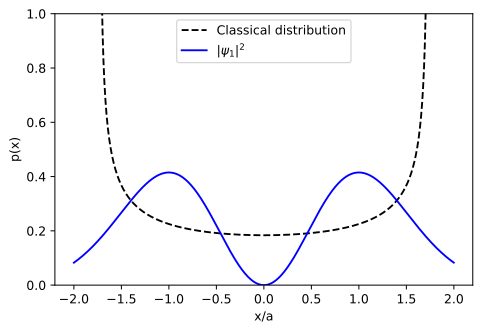
\includegraphics[scale=0.7]{n1.png}}
  \caption{Graph comparing the probability distributions of a SHO and QHO at quantum number $n=1$.}
  \label{fig:n1}
\end{figure}

However, when we approach sufficiently large quantum numbers, we see Bohr's principle emerge, and the quantum distribution closely follows the classical distribution.
\begin{figure}[h!]
  \centering
  \begin{subfigure}{.5\textwidth}
    \centering
    \centerline{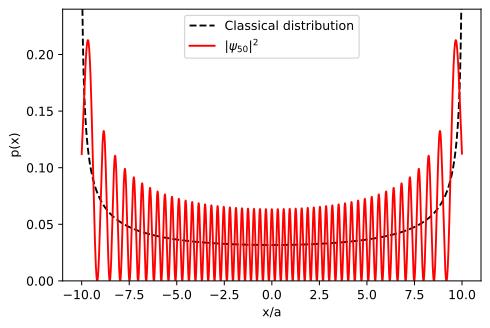
\includegraphics[scale=0.55]{n50.png}}
    \caption{{\lstinline$n=50$}}
  \end{subfigure}%
  \begin{subfigure}{.5\textwidth}
    \centering
    \centerline{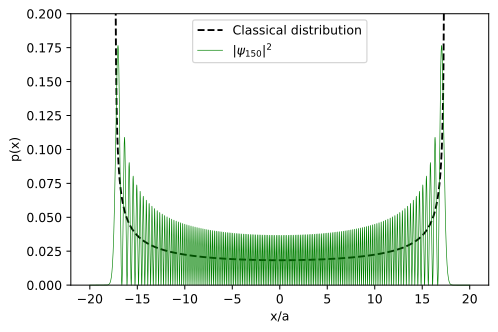
\includegraphics[scale=0.55]{n150.png}}
    \caption{{\lstinline$n=150$}}
  \end{subfigure}
  \label{fig:gratings}
  \caption{Graphs comparing the probability distributions of a SHO and QHO at quantum numbers $n=50$ and $n=150$.}
  \end{figure}
\newpage
From these graphs, we can conclude that the classical harmonic oscillator approximates a quantum harmonic oscillator at sufficiently large quantum numbers, as described by Bohr's correspondence principle.
\newpage

\begin{appendix}
\section{Python Code for Wave Functions}\label{sec:python}
\lstinputlisting[language=Python,frame=single]{py.py}
\newpage
\bibliographystyle{plainnat}
\bibliography{export}

\end{appendix}


\end{document}